{\bfseries
	Pour cette première partie, aucune justification n'est demandée et une seule réponse est possible par question.

	Pour chaque question, reportez son numéro sur votre copie et indiquez votre réponse.}

	Une réponse fausse ou l'absence de réponse n'enlève aucun point.

\subsection*{Question 1}

	Augmenter un nombre de 4\,\% revient à le multiplier par :

\begin{center}
	\begin{tblr}{hlines, vlines, colspec = {*4{X[c]}}}
		\textbf{A.}\quad {$0{,}04$}&
		\textbf{B.}\quad {$0{,}4$}&
		\textbf{C.}\quad {$1{,}04$}&
		\textbf{D.}\quad {$1{,}4$}\\
	\end{tblr}
\end{center}

\subsection*{Question 2}

	25\,\% de 80 est égal à :

	\begin{center}
	\begin{tblr}{hlines, vlines, colspec = {*4{X[c]}}}
		\textbf{A.}\quad {$16$}&
		\textbf{B.}\quad {$20$}&
		\textbf{C.}\quad {$60$}&
		\textbf{D.}\quad {$100$}\\
	\end{tblr}
	\end{center}

\subsection*{Question 3}

	Trois quarts d'heure correspondent à :

	\begin{center}
	\begin{tblr}{hlines, vlines, colspec = {*4{X[c]}}}
		\textbf{A.}\quad 15 minutes&
		\textbf{B.}\quad 40 minutes&
		\textbf{C.}\quad 45 minutes&
		\textbf{D.}\quad 75 minutes\\
	\end{tblr}
	\end{center}

\subsection*{Question 4}

	Le nombre $4{,}31 \times 10^{-5}$ peut s'écrire :

	\begin{center}
	\begin{tblr}{hlines, vlines, colspec = {*4{X[c]}}}
		\textbf{A.}\quad {$0{,}000\,043\,1$}&
		\textbf{B.}\quad {$0{,}000\,431$}&
		\textbf{C.}\quad {$0{,}004\,31$}&
		\textbf{D.}\quad {$431\,000$}\\
	\end{tblr}
	\end{center}

\subsection*{Question 5}

	On donne $V = \pi h R^{2}$ avec $h = 4$, $R = 5$ et $\pi \approx 3{,}14$. \\
	Un calcul numérique permettant d'obtenir une valeur approchée de $V$ est :

	\begin{center}
	\begin{tblr}{hlines, vlines, colspec = {*4{X[c]}}}
		\textbf{A.}\quad {$3{,}14 \times 4 \times 25$}&
		\textbf{B.}\quad {$3{,}14 \times (4 \times 5)^{2}$}&
		\textbf{C.}\quad {$(3{,}14 \times 4 \times 5)^{2}$}&
		\textbf{D.}\quad {$3{,}14 \times 4 \times 5$}\\
	\end{tblr}
	\end{center}

\subsection*{Question 6}
	On donne les deux graphiques ci-dessous :

	\begin{center}
	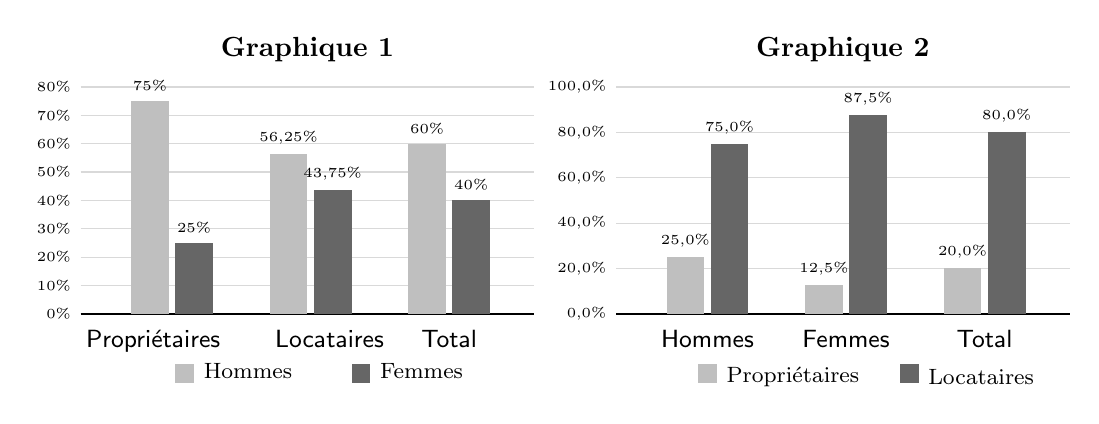
\begin{tikzpicture}[scale=0.8]
		
		\begin{scope}[xshift=0cm]
			\foreach \y in {0,10,...,80} {
				\draw[gray!30] (0,\y*0.045) -- (7.2,\y*0.045);
				\node[left, font=\tiny] at (0,\y*0.045) {\y\%};
			}
			\draw[line width=0.6pt] (0,0) -- (7.2,0);

			
			\fill[gray!50] (0.8,0) rectangle (1.4,75*0.045);
			\node[above, font=\tiny] at (1.1,75*0.045) {75\%};
			\fill[gray!80!black] (1.5,0) rectangle (2.1,25*0.045);
			\node[above, font=\tiny] at (1.8,25*0.045) {25\%};
			\node[below, font=\sffamily\small] at (1.15,-0.1) {Propriétaires};

			
			\fill[gray!50] (3.0,0) rectangle (3.6,56.25*0.045);
			\node[above, font=\tiny] at (3.3,56.25*0.045) {56,25\%};
			\fill[gray!80!black] (3.7,0) rectangle (4.3,43.75*0.045);
			\node[above, font=\tiny] at (4.0,43.75*0.045) {43,75\%};
			\node[below, font=\sffamily\small] at (3.95,-0.1) {Locataires};

			
			\fill[gray!50] (5.2,0) rectangle (5.8,60*0.045);
			\node[above, font=\tiny] at (5.5,60*0.045) {60\%};
			\fill[gray!80!black] (5.9,0) rectangle (6.5,40*0.045);
			\node[above, font=\tiny] at (6.2,40*0.045) {40\%};
			\node[below, font=\sffamily\small] at (5.85,-0.1) {Total};

			\node[font=\bfseries] at (3.6,4.2) {Graphique 1};

			
			\fill[gray!50] (1.5,-0.8) rectangle (1.8,-1.1);
			\node[right, font=\footnotesize] at (1.8,-0.9) {Hommes};
			\fill[gray!80!black] (4.3,-0.8) rectangle (4.6,-1.1);
			\node[right, font=\footnotesize] at (4.6,-0.9) {Femmes};
		\end{scope}

		
		\begin{scope}[xshift=8.5cm]
			\foreach \y in {0,20,...,100} {
				\draw[gray!30] (0,\y*0.036) -- (7.2,\y*0.036);
				\node[left, font=\tiny] at (0,\y*0.036) {\np{\y},0\%};
			}
			\draw[line width=0.6pt] (0,0) -- (7.2,0);

			
			\fill[gray!50] (0.8,0) rectangle (1.4,25*0.036);
			\node[above, font=\tiny] at (1.1,25*0.036) {25,0\%};
			\fill[gray!80!black] (1.5,0) rectangle (2.1,75*0.036);
			\node[above, font=\tiny] at (1.8,75*0.036) {75,0\%};
			\node[below, font=\sffamily\small] at (1.45,-0.1) {Hommes};

			
			\fill[gray!50] (3.0,0) rectangle (3.6,12.5*0.036);
			\node[above, font=\tiny] at (3.3,12.5*0.036) {12,5\%};
			\fill[gray!80!black] (3.7,0) rectangle (4.3,87.5*0.036);
			\node[above, font=\tiny] at (4.0,87.5*0.036) {87,5\%};
			\node[below, font=\sffamily\small] at (3.65,-0.1) {Femmes};

			
			\fill[gray!50] (5.2,0) rectangle (5.8,20*0.036);
			\node[above, font=\tiny] at (5.5,20*0.036) {20,0\%};
			\fill[gray!80!black] (5.9,0) rectangle (6.5,80*0.036);
			\node[above, font=\tiny] at (6.2,80*0.036) {80,0\%};
			\node[below, font=\sffamily\small] at (5.85,-0.1) {Total};

			\node[font=\bfseries] at (3.6,4.2) {Graphique 2};

			
			\fill[gray!50] (1.3,-0.8) rectangle (1.6,-1.1);
			\node[right, font=\footnotesize] at (1.6,-1) {Propriétaires};
			\fill[gray!80!black] (4.5,-0.8) rectangle (4.8,-1.1);
			\node[right, font=\footnotesize] at (4.8,-1) {Locataires};
		\end{scope}
	\end{tikzpicture}
	\end{center}



































































	La proportion d'hommes parmi les locataires est :

	\begin{center}
	\begin{tblr}{hlines, vlines, colspec = {*4{X[c]}}}
		\textbf{A.}\quad {$25{,}0\,\%$}&
		\textbf{B.}\quad {$43{,}75\,\%$}&
		\textbf{C.}\quad {$56{,}25\,\%$}&
		\textbf{D.}\quad {$75{,}0\,\%$}\\
	\end{tblr}
	\end{center}

\subsection*{Question 7}
	Sur $\R$, l'équation $6x-5=4x+3$ a pour solution :

\begin{center}
	\begin{tblr}{hlines, vlines, colspec = {*4{X[c]}}}
		\textbf{A.}\quad {$x=-2$}&
		\textbf{B.}\quad {$x=1$}&
		\textbf{C.}\quad {$x=2$}&
		\textbf{D.}\quad {$x=4$}\\
	\end{tblr}
\end{center}

\subsection*{Question 8}


	La droite $(\Delta)$ est la représentation graphique d'une fonction affine $f$ définie sur $\R$.

\begin{center}
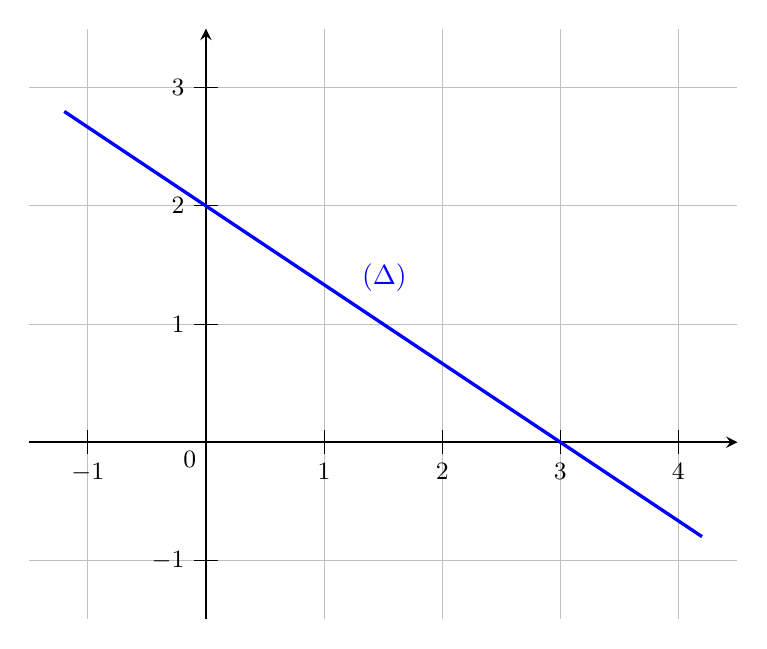
\begin{tikzpicture}[scale=1.5, baseline={(current bounding box.center)}]
	\draw[gray!50, line width=0.4pt] (-1.5,-1.5) grid (4.5,3.5);
	\draw[line width=0.8pt,->,>=stealth] (-1.5,0) -- (4.5,0);
	\draw[line width=0.8pt,->,>=stealth] (0,-1.5) -- (0,3.5);
	\foreach \x in {-1,1,2,3,4}
		\draw (\x,0.1) -- (\x,-0.1) node[below, font=\small]{$\np{\x}$};
	\foreach \y in {-1,1,2,3}
		\draw (0.1,\y) -- (-0.1,\y) node[left, font=\small]{$\np{\y}$};
	\node[below left, font=\small] at (0,0) {$0$};
	\draw[line width=1.2pt, color=blue] (-1.2,2.8) -- (4.2,-0.8) node[pos=0.45, above right]{\blue $(\Delta)$};
\end{tikzpicture}
\end{center}













	L'expression de $f$ est :

\begin{center}
	\begin{tblr}{hlines, vlines, colspec = {*4{X[c]}}}
		\textbf{A.}\quad {$f(x)=2x+3$}&
		\textbf{B.}\quad {$f(x)=3x+2$}&
		\textbf{C.}\quad {$f(x)=-\dfrac{3}{2}x+3$}&
		\textbf{D.}\quad {$f(x)=-\dfrac{2}{3}x+2$}\\
	\end{tblr}
\end{center}
